% Created 2021-09-27 Mon 12:01
% Intended LaTeX compiler: xelatex
\documentclass[letterpaper]{article}
\usepackage{graphicx}
\usepackage{grffile}
\usepackage{longtable}
\usepackage{wrapfig}
\usepackage{rotating}
\usepackage[normalem]{ulem}
\usepackage{amsmath}
\usepackage{textcomp}
\usepackage{amssymb}
\usepackage{capt-of}
\usepackage{hyperref}
\setlength{\parindent}{0pt}
\usepackage[margin=1in]{geometry}
\usepackage{fontspec}
\usepackage{svg}
\usepackage{cancel}
\usepackage{indentfirst}
\setmainfont[ItalicFont = LiberationSans-Italic, BoldFont = LiberationSans-Bold, BoldItalicFont = LiberationSans-BoldItalic]{LiberationSans}
\newfontfamily\NHLight[ItalicFont = LiberationSansNarrow-Italic, BoldFont       = LiberationSansNarrow-Bold, BoldItalicFont = LiberationSansNarrow-BoldItalic]{LiberationSansNarrow}
\newcommand\textrmlf[1]{{\NHLight#1}}
\newcommand\textitlf[1]{{\NHLight\itshape#1}}
\let\textbflf\textrm
\newcommand\textulf[1]{{\NHLight\bfseries#1}}
\newcommand\textuitlf[1]{{\NHLight\bfseries\itshape#1}}
\usepackage{fancyhdr}
\pagestyle{fancy}
\usepackage{titlesec}
\usepackage{titling}
\makeatletter
\lhead{\textbf{\@title}}
\makeatother
\rhead{\textrmlf{Compiled} \today}
\lfoot{\theauthor\ \textbullet \ \textbf{2021-2022}}
\cfoot{}
\rfoot{\textrmlf{Page} \thepage}
\renewcommand{\tableofcontents}{}
\titleformat{\section} {\Large} {\textrmlf{\thesection} {|}} {0.3em} {\textbf}
\titleformat{\subsection} {\large} {\textrmlf{\thesubsection} {|}} {0.2em} {\textbf}
\titleformat{\subsubsection} {\large} {\textrmlf{\thesubsubsection} {|}} {0.1em} {\textbf}
\setlength{\parskip}{0.45em}
\renewcommand\maketitle{}
\author{Houjun Liu}
\date{\today}
\title{DNA Replication}
\hypersetup{
 pdfauthor={Houjun Liu},
 pdftitle={DNA Replication},
 pdfkeywords={},
 pdfsubject={},
 pdfcreator={Emacs 28.0.50 (Org mode 9.4.4)}, 
 pdflang={English}}
\begin{document}

\tableofcontents



\section{DNA Replication}
\label{sec:org3f50245}
DNA replication is known to be "semi-conservative" --- meaning that it
is a process that pairs a synthesized half of the DNA with an original
half of the DNA (i.e. takes the ORIGINAL template strand + makes the NEW
coding strand \& takes the ORIGINAL coding strand + makes the NEW
template strand.)

Because \textbf{polymerases copy uni-directionally} => DNA polyemrease move
along the 3' to 5' DNA to create a copy 5' to 3'. Meaning, the
polymerize is able to add nucleotide onto the 3' end of the DNA.

As mentioned before, \textbf{DNA Polymerease} is the enzyme that catalyzes this
process of DNA replication.

\subsection{The Process of DNA Replication}
\label{sec:org6b1407c}
\subsubsection{DNA Unzipping}
\label{sec:org3ddd46a}
=> DNA is unzipped at the origin of replication The parent DNA strand
serves as a template for the new strand; when it is unzipped, the
nucleotides are exposed for complementary base pairing. \textbf{Helicase} is
the enzyme that unzips the DNA molecule, breaking the hydrogen bonds
between nucleotides to expose them for complementary base pairing

\subsubsection{DNA priming}
\label{sec:org13af20f}
DNA polymersease will REQUIRE a double-stranded area to begin work from,
so \textbf{Primase} synthesize already double-stranded RNA primers that DNA
polymerease could bootstrap to the single-stranded DNA to begin the
replication process (think: create-react-app)

\subsubsection{DNA "flexing" (what's the actual word?)}
\label{sec:org9114e81}
The primed DNA is broken and rejoined in order to reduce strain caused
by unzipping. Topoisomerase is responsible for relieving
unwinding-induced.

\subsubsection{The actual process of replication}
\label{sec:org9234398}
In this step, DNA polymerease does we came here to do.

Because DNA polymerase could only add nucleotides 5' to 3', there is two
types of styles of copying depending on which of the two strands are
being copied.

\begin{itemize}
\item In the \textbf{leading} strand (3' to 5'), polymerase will run alongside the
helicase for they are opening and replicating on the same direction
\item In the \textbf{lagging} strand (5' to 3'), polymerase will wait until the
helicate opens a little segment, and rushes forward and move backwards
\end{itemize}

/NOTE: the lagging strand\ldots{} 1) takes longer to transcribe 2) is done in
small chunks (each "rush forward"). Each chunk is called an ogazaki
fragment --- this is why there was that
\href{KBhBIO101mRNAPreprocessing.org}{KBhBIO101mRNAPreprocessing}
process during transcription because that would help correct any errors
in joining these fragments/

\begin{figure}[htbp]
\centering
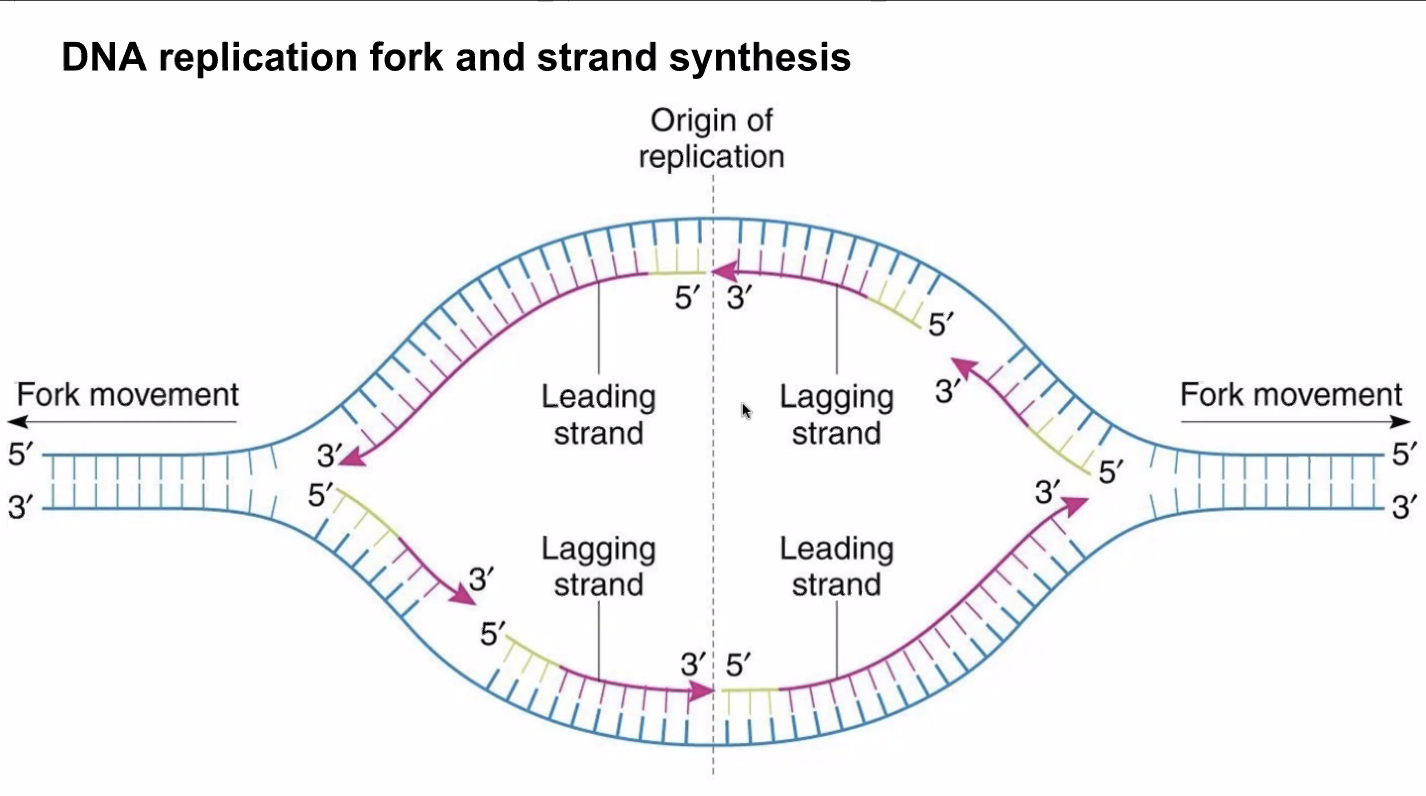
\includegraphics[width=.9\linewidth]{leadinglagging.png}
\caption{leadinglagging.png}
\end{figure}

\noindent\rule{\textwidth}{0.5pt}

\emph{A quick break\ldots{}}

But where does the materials (the nucleotide necessary to make new DNA +
primer RNA come from?)

Remember that this whole process happens in the nucleus. There's
apparently just a crap tonne of random nucleotide floating around in the
nucleus, so simple chemical attraction is good enough. \textbf{*}

\subsubsection{DNA Proofreading}
\label{sec:org0789e40}
DNA polymerse will detect unfitting bonds and remove leftover RNA primer
bootstrap units to repair them in a process called "proofreading." DNA
polimersease is assisted with "glue" ligase to help the DNA polymerease
pick out and replace problematic/unneeded nucleotides and perhaps their
neighbors. This is where the Ogazaki fragments get joined.

Steps of DNA replication, in Paul's words:

\begin{verbatim}
- Many proteins work together in DNA replication and repair. 
The process of DNA replication is semiconservative, such that takes place through complementary base pairing of a template strand of parent DNA. 

- The process of replication begins at the origin of replication, forming a replication fork. The enzyme, helicase, unwinds DNA exposing template strands, primase synthesizes RNA primers to begin the process

- Topoisomerase breaks, swivels, and rejoins the parent DNA to relieve strain caused by unwinding. 

- DNA polymerase is the enzyme that catalyzes the process of complementary base pairing of nucleotides to the template strand. 

- New nucleotide strands always for in the 5’ to 3’ direction, therefore the leading strand forms continuously but the lagging strand is formed in Okazaki fragments (still in the 5’ to 3’ direction) and connected by the enzyme ligase. 

- DNA polymerase is able to proofread pairing, and along with mismatch repair enzymes, DNA is carefully check and repair DNA. 

- The end of a DNA molecule are called telomeres (not in circular genome e.g. bacteria), and shorten during each replication (Hayflick limit). Noncoding, repeating units of nucleotides act as protection from losing essential genetic information by shorting. 
\end{verbatim}

\begin{figure}[htbp]
\centering
\includegraphics[width=.9\linewidth]{copying 1.png}
\caption{copying 1.png}
\end{figure}

\noindent\rule{\textwidth}{0.5pt}
\end{document}
